%% Los cap'itulos inician con \chapter{T'itulo}, estos aparecen numerados y
%% se incluyen en el 'indice general.
%%
%% Recuerda que aqu'i ya puedes escribir acentos como: 'a, 'e, 'i, etc.
%% La letra n con tilde es: 'n.


\chapter{Introducción}

El hombre ha desarrollado el mejoramiento vegetal en forma sistemática desde la aparición de la agricultura y lo ha convertido en un instrumento esencial para la mejora de la producción agrícola en términos de cantidad, calidad y diversidad. Se puede deducir claramente que la sociedad es la beneficiaria del trabajo de fitomejoramiento, debido a que su principal finalidad es obtener mejores resultados de la actividad agrícola, ya sea en alimentos, o en productos que luego serán utilizados en la industria. 

Las variedades mejoradas son el resultado del trabajo de desarrollo genético llevado a cabo en los programas de fitomejoramiento, los cuales se extienden a lo largo de varios años y requieren cuantiosas inversiones. La vigencia comercial de las variedades puede extenderse varias décadas, por lo que su elección es crítica para que el productor evite pérdidas económicas por malas campañas y el suministro al mercado sea constante. 

La selección de genotipos de buen rendimiento y estabilidad se realiza mediante el análisis de datos provenientes de ensayos multiambientales(EMA), esenciales para analizar la estabilidad del rendimiento. Los EMA comprenden experimentos en múltiples ambientes y son herramientas fundamentales para incrementar la productividad y rentabilidad de los cultivos.

Debido a que las regiones de producción de los principales cultivos cubren áreas ecológicas muy extensas, se observan variaciones en las condiciones climaticas y de suelo, y la aparición de la interacción genotipo ambiente (IGA) es inevitable, provocando respuestas altamente variables. La IGA es considerada casi unánimemente por los fitomejoradores como el
principal factor que limita la respuesta a la selección y, en general, la eficiencia de los programas de mejoramiento.  
La IGA se puede visualizar al comparar, por ejemplo, el rendimiento de los genotipos en dos ambientes diferentes. Cuando dos genotipos X e Y tienen una respuesta diferencial en ambos ambientes, pero su ordenación permanece sin cambios se dice que la interaccion es no crossover (Figura 1(A)). Sin embargo, la interacción es de tipo crossover cuando hay cambios en el orden de los genotipos (Figura  1(B)). Cuando los genotipos responden de manera similar en ambos ambientes (Figura 1(C)) no hay IGA. 

\begin{figure}[h]
\begin{center}
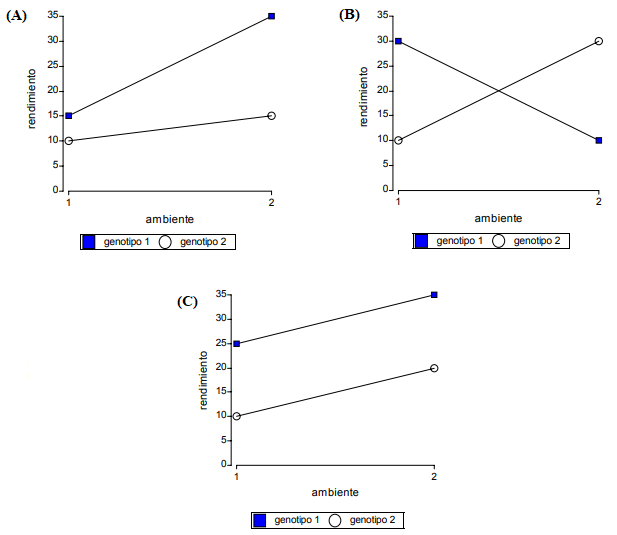
\includegraphics[width=14cm]{./Graficos/figura1}
\end{center}
\caption{Representación gráfica de tipos de IGA: (A)IGA no crossover, (B) IGA crossover y (C) no IGA}
\end{figure}


Distintos conceptos como regiones ecológicas, ecotipos, mega-ambientes, adaptación específica y estabilidad se pueden analizar a partir de la interacción genotipo-ambiente (Yan y Hunt, 2001).


Comprender la relación entre el rendimiento del cultivo y el medio ambiente ha sido durante mucho tiempo una clave problema para los fitomejoradores y genetistas. El rendimiento del cultivo, el fenotipo observado, es una función de genotipo (G): variedad o cultivar, medio ambiente (A) y IGA. En general, el rendimiento se puede expresar de la siguiente manera si la interacción entre G y E es significativa:
\begin{center}
$R=G+A+IGA$
\end{center}


Los investigadores agrícolas han sido conscientes de las diversas implicaciones de IGA en los programas de mejoramiento (Mooers, 1921; Yates y Cochran, 1938). Por ejemplo, la IGA tiene un impacto negativo en la heredabilidad, cuanto menor sea la heredabilidad de un caracter, mayor será la dificultad para mejorar ese caracter mediante la selección.
Por lo tanto, información sobre la estructura y la naturaleza de la IGA es particularmente útil para los mejoradores porque puede ayudar a determinar si necesitan desarrollar cultivares para todos los ambientes de interés o si deberían desarrollar cultivares específicos para ambientes específicos (Bridges, 1989). Gauch y Zobel (1996) explicaron la importancia de IGA como: “Si no hubiera interacción, una sola variedad de trigo (\emph{Triticum aestivum} L.) o maíz (\emph{Zea mays} L.) o cualquier otro cultivo rendiria al máximo en todo el mundo, y además la prueba de variedades deberia realizarse en un sólo lugar para proporcionar resultados universales. No habría ruido, los resultados experimentales serían exactos, identificando la mejor variedad sin error, y no habría necesidad de replicación. Entonces, una réplica en un lugar identificaría la mejor variedad de trigo que florece en todo el mundo ".


Un análisis adecuado de la información de los EMA es indispensable para que el programa de mejoramiento de los cultivos sea eficaz. El rendimiento medio en los ambientes es un indicador suficiente del rendimiento genotípico solo en ausencia de IGA(Yan y Kang, 2003). Sin embargo, la aparición de IGA es inevitable y no basta con la comparación de las medias de los genotipos, sino que se debe recurrir a una metodología estadística más aporopiada. Entre los métodos más difundidos para analizar los datos provenientes de EMA se encuentran los modelos de regresión, análisis de variancia y técnicas de análisis multivariado. 

Para analizar la IGA se han propuesto varios métodos a través de los años. En 1938 Yates y Cochran trataron de interpretar la interacción calculando la regresión de las medias genotípicas en las medias ambientales, calculadas tomando el promedio de todos los genotipos en ese ambiente. Posteriormente Finlay y Wilkinson (1963) y Eberhart y Russell (1966) retomaron esta práctica, pero con enfoques diferentes.

Shukla (1972) y Cruz Medina (1992) proponen un método práctico para estimar la componente de la interacción GA correspondiente a cada genotipo, incluyendo la posibilidad de efectuar test de hipótesis y permitiendo una posterior extensión del modelo en la interpretación de la inestabilidad. Para ello se considera alguna característica ambiental medible como covariable. Este método también se puede aplicar a los ambientes.

En los últimos años, dos modelos multiplicativos, el modelo de los efectos principales aditivos y interacción multiplicativa (AMMI, \emph{Additive Main effects and Multiplicative Interaction}) y el de regresión por sitio (SREG), han aumentado su popularidad entre los fitomejoradores como una herramienta de análisis gráfico. Estos modelos combinan el análisis de varianza (ANOVA) y la descomposición de valores singulares (SVD) o el análisis de componentes principales (PCA) en la matriz residual de ANOVA. En SREG, el ANOVA se realiza sobre el efecto principal de A mientras que en AMMI se considera el efecto de G y A. 


En este contexto, el análisis de datos provenientes de ensayos multiambientales requiere metodología estadística sofisticada cuyas rutinas informáticas se encuentran disponibles en programas desarrollados por diferentes empresas. Esto genera el inconveniente de tener que disponer de todos los programas necesarios para los distintos análisis, atender los requerimientos de formatos de datos usados por cada uno, y comprender los diversos tipos de salidas en las que se ofrecen los resultados obtenidos. Además, algunos procedimientos, especialmente aquellas metodologías recientes, no se encuentran dispobibles, y los costos de las licencias de dichos programas resultan muy elevados. De aqui surge la necesidad de disponer de algún software libre que contemplara la mayoría de las rutinas necesarias para analizar los datos provenientes de EMA. Este problema, puede ser resulto a partir del software R el cual es un lenguaje de programación interpretado. Se trata de un proyecto de software libre distribuido bajo los términos de la \emph{General Public Licence} (GNU). Es el resultado de la implementación del lenguaje S, uno de los lenguajes más utilizados en investigación por la comunidad estadística. A diferencia de otros programas de estadística usuales en el campo de la investigación, R no dispone de una interfaz gráfica con la cual se pueda realizar cualquier análisis, lo cual genera que muchos científicos no lo utilicen. Sin embargo, al tratarse de un lenguaje de programación, las posibilidades que ofrece en cuanto a la manipulación y análisis de los datos es mucho más vasta, ya que los usuarios pueden definir sus propias funciones, personalizar el tipo de análisis que quieren correr y, a largo plazo, hacer más rápido y eficiente este tipo de tarea. 

Una de las características de R es que promueve el hecho de que si alguien crea algo que considera útil para la comunidad pueda ponerlo al alcance de los demas usuarios.  Muchas veces, una función creada por algun usuario no resulta sencilla de reutilizar, por lo que se ha introducido la posibilidad de crear paquetes o librerías. 
Una librería o paquete (\emph{package}) es una colección de objetos creados y organizados siguiendo un protocolo fijo que garantiza un soporte mínimo para el usuario así como la ausencia de errores (de sintaxis) en la programación.
Al abrir R se cargan automáticamente una serie de paquetes básicos, como por ejemplo, \emph{base} o \emph{stats}, que contiene las funciones \emph{lm} o \emph{glm}. Sin embargo, R tiene paquetes (unos cuantos miles en la actualidad) . 

Al ser un software libre los usuarios tienen la libertad de ejecutar, copiar, distribuir, estudiar, modificar y mejorar el software. Más precisamente, software libre significa que los usuarios de un programa tienen las cuatro libertades esenciales:
\begin{enumerate}
\item Ejecutar el programa como lo desee, con cualquier propósito.
\item Estudiar el funcionamiento del programa y modificarlo de modo que realice las tareas que desee. El acceso al código fuente es un prerrequisito para esto.
\item Redistribuir copias para ayudar a los demás.
\item Distribuir copias de sus versiones modificadas a otras personas. Al hacerlo da a toda la comunidad la oportunidad de beneficiarse de sus cambios. El acceso al código fuente es un prerrequisito para esto.
\end{enumerate}

La comunidad de usuarios que programan en R ha ido creciendo notablemente en los últimos años y, al ser un software libre, han ido proporcionando librerías que extienden sus funciones básicas y pueden resultar realmente valiosas (casi indispensables). Entre ellas se encuentran, \emph{plyr}, \emph{lubridate}, \emph{reshape2} y \emph{stringr} para la manipulación de los datos; \emph{ggplot2} y \emph{rgl} para la visualización; \emph{knitr} y \emph{xtable} para la presentación de resultados; entre otros. La lista completa de los paquetes oficiales puede consultarse en CRAN\footnote{CRAN (Comprehensive R Archve Network) es el repositorio oficial de paquetes de R, el lugar donde se publican las nuevas versiones del programa, etc. Contiene la lista completa de paquetes oficiales. \url{https://cran.r-project.org/web/packages/available_packages_by_name.html}}. Además de los oficiales, existen paquetes que pueden instalarse desde repositorios como, por ejemplo, Github. Sin embargo, no es sencillo encontrar un paquete que puede ser útil para un determinado fin sino que se debe recurrir a varios de ellos para cumplir un determinado objetivo. 

Frecuentemente, los mejoradores utilizan una interfaz gráfica para realizar los análisis estadísticos deseados y no tienen un manejo fluido de un lenguaje de programación. En el año 2012 se creó el paquete \emph{Shiny} de RStudio, el cual permite desarrollar aplicaciones Web. En este sentido el paquete Shiny surge como una útil y versátil herramienta que permite acercar la potencia de R a todo tipo de usuarios.

El objetivo del presente trabajo fue: (i) crear un paquete de R que incluya las funciones que permitan analizar la interacción genotipo por ambiente, incluyendo además metodología recientemente publicada que no se encuentra disponible en R; (ii) crear una interfaz gráfica, entre R y el usuario, mediante Shiny que permita realizar los análisis disponibles en el paquete creado.



